\chapter{Introduction}
%%Introduction %%%%
\section{Motivation}
Today, combustion processes are the power horse of the world's transport and energy production systems and in some areas such has aeronautics and fossil fuel power plants, due to their high efficiency, high thrust to weight ratios and fast response times, they are irreplaceable in the power gap from several hundred kilowatt to hundreds of megawatt. The problem is even more acute in rocket propulsion, where the demand is in the order of the gigawatt \cite{nato}.

\begin{figure}[!htb]
	\begin{subfigmatrix}{2}
	\subfigure[GEnx turbofan engine cutaway.]{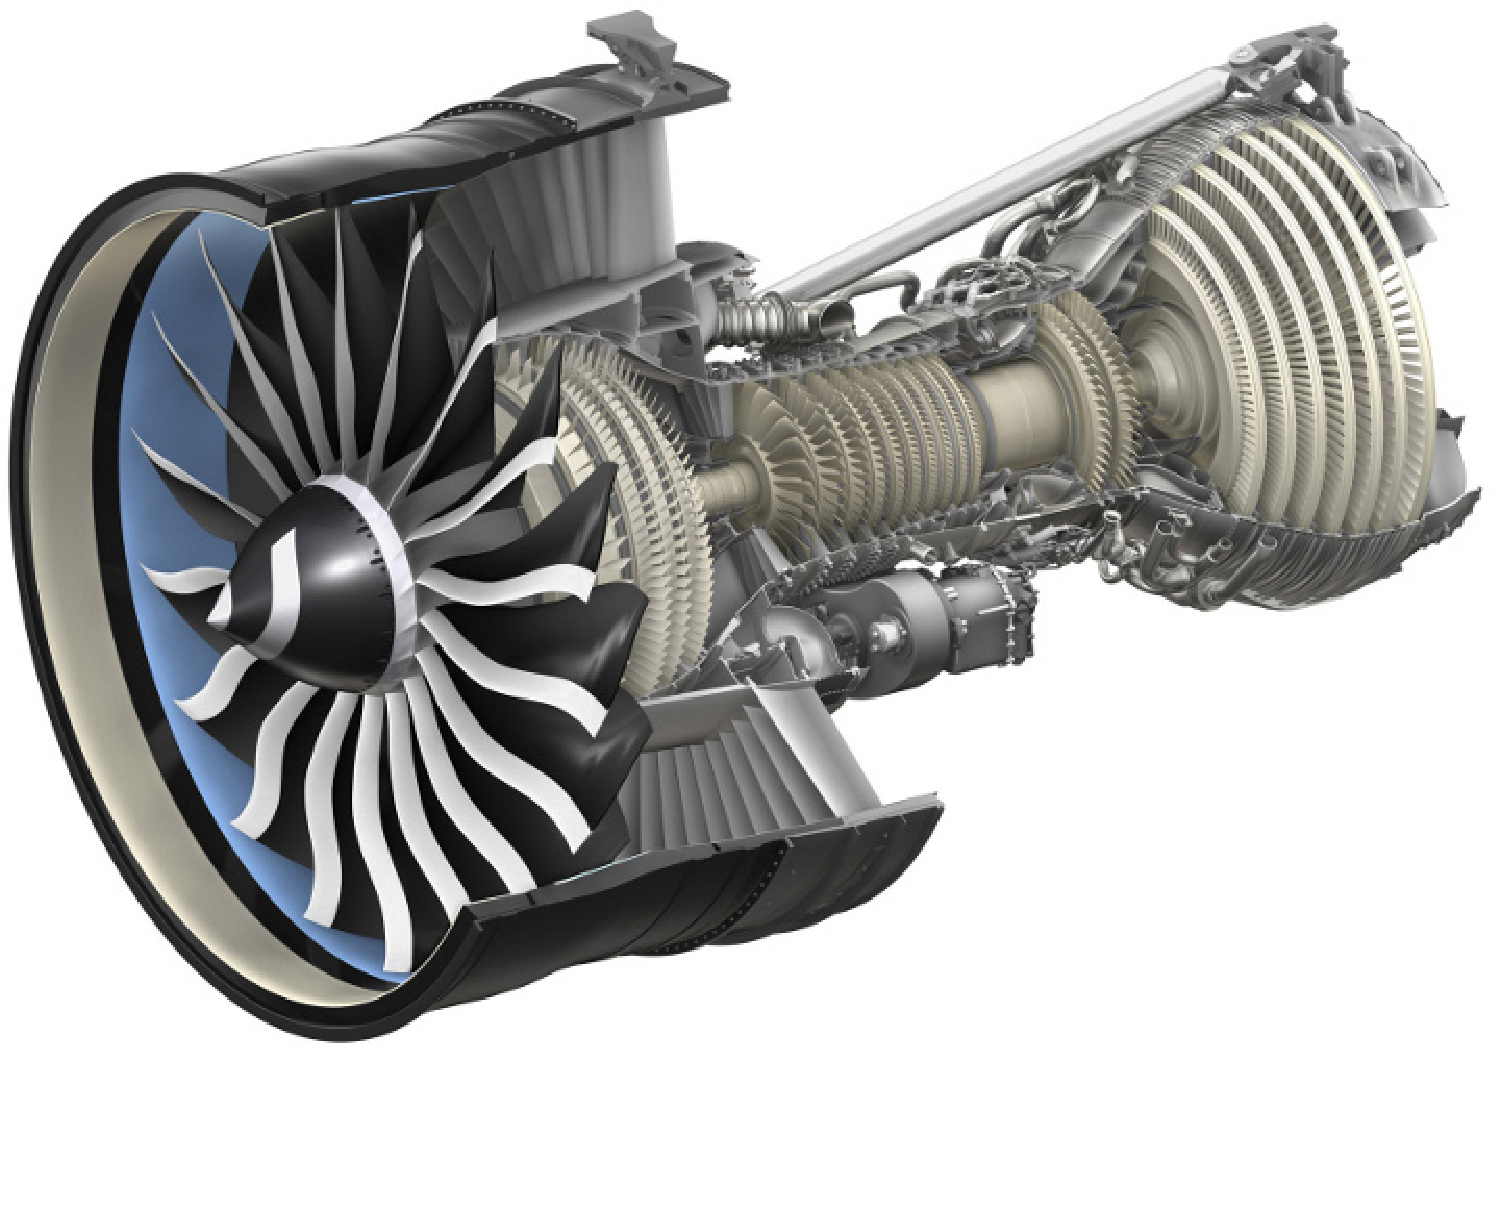
\includegraphics[width=0.49\linewidth]{./img/GEnx_engine}\label{turbofan_eng}}
	\subfigure[NASA J-2X upper stage rocket engine.]{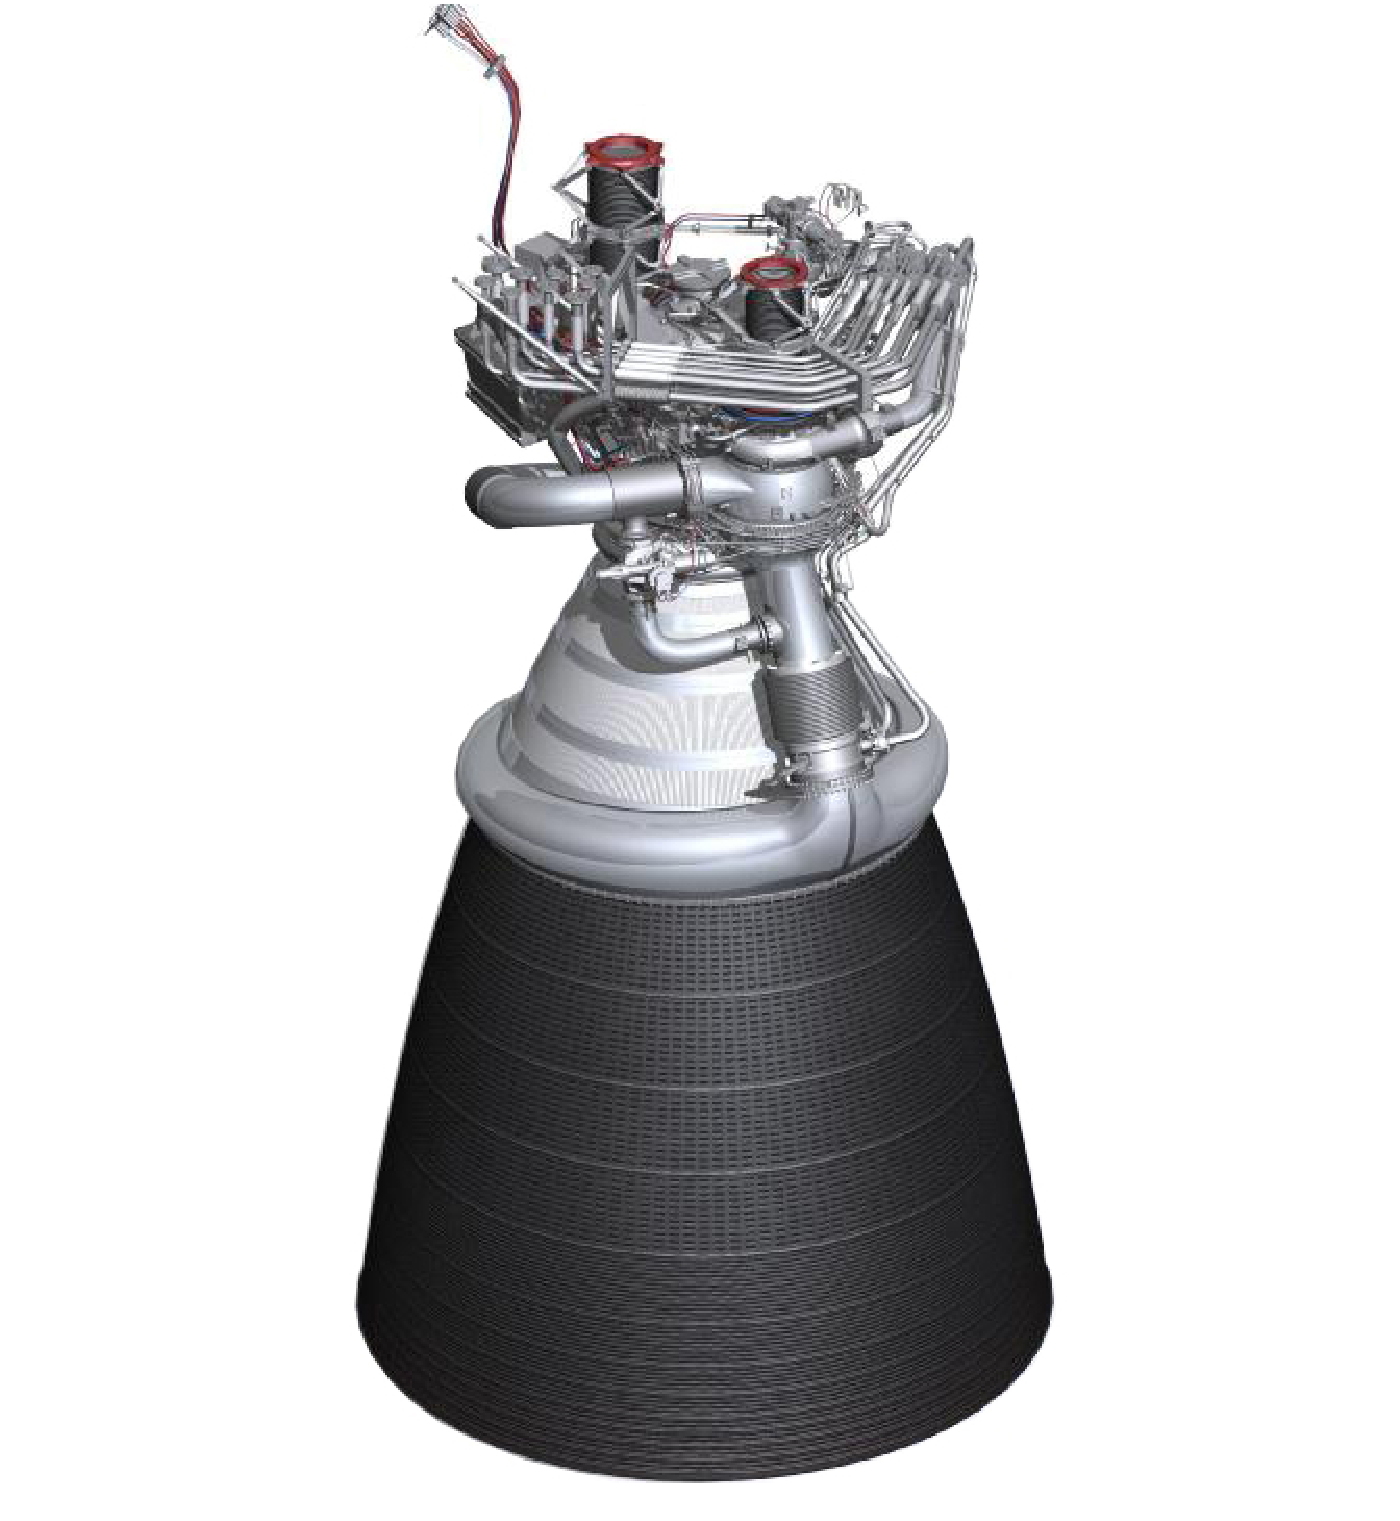
\includegraphics[width=0.49\linewidth]{./img/NASA_J2X_engine}\label{rocket_eng}}
	\end{subfigmatrix}
	\caption{Examples of modern combustion systems on which there are no reliable technological alternatives, and where combustion instabilities are a limiting performance factor.\comment{referenciar imagens}}
	\label{engines}
\end{figure}


The demand for evermore efficient, and less pollutant, specially on $NO_x$ emission, has pushed the design of some systems toward leaner and in if possible premixed combustion. Operating at lower temperatures and in conditions closer to the flammability or blowout limit, tends to aggravate the combustion instabilities \cite{candel}, \cite{lefebvre}, \cite{ghoniem}, that usually results in excessive vibrations, mechanical faults, high levels of acoustic noise, high burn and heat transfer rates possibly melting the components, therefore extremely undesirable,\cite{prateep}.
This is the more or less the motivation behind all combustion instability studies, however the topic is complex, far from well defined and therefore very broad.  We start with a brief revision of the combustion instabilities, then focus on the thermoacoustic instabilities, then link them to the G-equation formulation, a level set method for flame kinematics. During those steps we hope to make clear the areas of concern of our specific approach, as well try to frame it in wider context.

% INSERT BULLETS


\newpage 
\section{Combustion Instabilities Revision}
Upon the bibliographic revision of combustion instabilities, several different definition arose, most of them were in fact specific to a certain type instability. The most global approaches were given by \cite{candel} and by \cite{barrere},  and a conceptual summary is presented in figure \ref{mindmap}.

%FIGURE
\begin{figure}[!htb]
	\begin{center}
	\includegraphics[scale=1.02]{./img/mindmap}
	\end{center}
	\caption{Illustrative mind-map of combustion instabilities. We present a conceptual classification according to \cite{barrere}, and also examples or mechanisms of instabilities in each category. The red circles represent the topics with this study will focus on, thermoacoustics and flame kinematics instability mechanisms. \comment{change kinematics to dynamics) improve visiability}}
	\label{mindmap}
\end{figure}


The conceptual representation of figure \ref{mindmap}, was progressively created has researchers focused their attention and analysis on only a small subset of mechanisms, that dominated their specific problem.
Thus we must emphasize that the conceptual categories of figure \ref{mindmap}, are in no way isolated.  On the contrary, real systems should be considered has a multivariate dynamical system coupling all the above mechanism, however not all with the same intensity.

An interesting perspective shown in figure \ref{mindmap}, and also described in \cite{barrere} is that the instabilities can be ordered by characteristic space scales where they develop. Intrinsic instabilities are not system dependent since the usually develop in the smaller space scales, such as the local flame front, or even smaller, the chemical reaction scales. In the combustion chamber instabilities some of major effects are driven by the fluid flow, acoustic or shock wave interactions inside the chamber. In a even larger space scales we have system instabilities, that act on space scale of the heater, engine, turbine, rocket or even in the entire launch vehicle.
These larger space scales of combustion instabilities drivers, can influence or be triggered by the lower ones thus creating a very complex interaction of cause's and effects.

In this report we restrict ourselves to thermoacoustic and flame kinematic coupling, and try to improve the models for application where these phenomena are the prime drivers of combustion instabilities. 

\section{Thermoacoustic Instabilities}
In a control theory analogy thermoacoustic instabilities are acoustic waves (pressure, velocity or density) coupled with heat release fluctuations. The major source of the heat release is the flame and thus it's kinematics strongly influence dynamical response of the system, as presented in figure \ref{feedback_combustion}, inspired by \cite{nato} and specially by \cite{ghoniem}.

\begin{figure}[h!]
\begin{center}
\includegraphics[scale=1.2]{./img/feedback_combustion}
\end{center}
\caption{Schematic diagram of thermoacoustic combustion instabilities as a feedback amplifier between acoustic waves, and heat release emanating from the flame front.}
\label{feedback_combustion}
\end{figure}

%The coupling of acoustics and heat release, was first experimentally detected by Rijke in 1859 by heating a metallic grid, inside a open ended tube, with a flame or with an electrical current (Joule effect), has shown in figure \ref{rijke_tube}. Under certain circumstances, the heat addiction generating a loud buzzing sound that emanated from the tube.

%\begin{figure}[h]
%\begin{center}
%\includegraphics[scale=1]{./img/rijke_tube}
%\end{center}
%\caption{Rijke's tube, that revealed the coupling of acoustics and heat. The metallic grid release heat, supplied by a flame or electric current, and thus in certain circumstances generates intense acoustic waves inside the pipe, that makes it resonate at is natural frequency.}
%\label{rijke_tube}
%\end{figure}
%However a solid explanation for the phenomena was due Lord Rayleigh (1877), along is foundation of the theory of sound, one of is corollaries (\emph{Rayleigh Criterion}) is a crucial tool in determining the presence of thermoacoustic instabilities in a given system. 

%\begin{corolary}[\bf{Rayleigh Criterion}]
%\begin{align*}
%\underbrace{\int\limits_T \int\limits_V p'(\vec{x},t) q'(\vec{x},t) dV dt}_{\substack{ acoustic\ energy\ generated \\ by\ heat\ sources}} \quad > \underbrace{\int\limits_T \int\limits_V \Phi(\vec{x},t) dV dt}_{\substack{acoustic\ energy\ dissipated\\by\ generalized\ sinks}} \Longrightarrow & \\[-21mm] & \; Thermoacoustic \\ & \quad \; \; \; Instability
%\end{align*}
%\end{corolary}
%\vspace{2cm}

%\clearpage
%\newpage
%\section{Flame Dynamic Instabilities}
%Flames are defined, at least according to \cite{turns}, as auto-sustained, relatively localized combustion wave. However flames are usually subdivided into premixed and non-premixed flames, in relation to the air-fuel mixture type, and also into laminar or turbulent flames, in relation to its dynamic properties. A classification of flames according to their configuration or type of burner from which they are generated is also common. 
%(ORDER BY: REGIME-laminar, TYPE-premixed, CONFIGURATION-bunsen)
%\subsection{Flame Regimes, Types and Configurations}
%Since there so many flame configurations and in so many fluid dynamic regimes, it is important for us to some how focus on subset which we consider of interest. The selection in our situation is a coalition of possible industrial application but also conditions that simplify the problem so that a more fundamental understanding could be grasped.
%Therefore we focus on {\bf\em Bunsen Premixed Laminar Flames}.



%Our study could be summed by \textbf{thermoacoustic driven instabilities}, and their \textbf{coupling with the flame kinematics}, of \textbf{laminar premixed flames} on \textbf{Bunsen burners}.

%Why \textbf{laminar} flow regime (as opposed to turbulent)?
%\begin{itemize}
%\item \small Simpler, and more accurate measurements of flow and flame properties
%\item \small Since $Da>>1$ we can assume zero thickness flame surface, and therefore apply G-equation Model directly
%\item \small Higher assurance of flame axisymmetry (turbulent flow tends to be 3D), and therefore simplify G-equation Model
%\item \small Simpler system enhances the ability to understand fundamental physical phenomena
%\item \small Laminar flame dynamics can be seen as building block for turbulent flames, such has in flamelet models
%\end{itemize}

%Why \textbf{premixed} flames (and not non-premixed or diffusion flames)?\\
%\begin{itemize}
%\item Reduces $NO_x$ emissions
%\item More fuel efficient
%\item However it's more susceptible to combustion instabilities
%\end{itemize}

%Why use \textbf{Bunsen burners}?
%\begin{itemize}
%\item \small Simple construction and operation
%\item \small Outlet flow is axisymmetric on laminar regime
%\item \small Outlet flow has almost uniform velocity profile
%\item \small Produces one single flame, thus not susceptible cross flame interaction 
%\end{itemize}


%\vspace{4mm}
%\noindent {\bf Why Laminar regime?} 
%\begin{itemize}
	%\item[$\blacktriangle$] Simplifies mathematical modeling. 
	%\item[$\blacktriangle$] Simplifies experimental measurements, with less fluctuations and chaotic behaviors.
	%\item[$\blacktriangledown$] Not directly applicable to turbulent flames.
	%\item[$\blacktriangle$] More fundamental knowledge is gained to produce enhanced models that could be used ``locally'', in turbulent flames (flamelet models).
%\end{itemize}
%\vspace{4mm}
%{\bf Why premixed flames?}
%\begin{itemize}
	%\item[$\blacktriangle$] Greatly reduces NOx, emissions.
	%\item[$\blacktriangle$] More fuel efficient. 
	%\item[$\blacktriangledown$] More susceptible to combustion instabilities. 
	%\item[$\blacktriangledown$] High risk of explosions in feed lines  
%\end{itemize}
%\vspace{4mm}
%{\bf Why Bunsen flame configuration?}
%\begin{itemize}
	%\item[$\blacktriangle$] Simple construction and operation.
	%\item[$\blacktriangle$] Growing application in industry.
	%\item[$\blacktriangle$] Outlet flow is axisymetric and on laminar regime.
	%\item[$\blacktriangle$] Outlet flow has uniform velocity profile.
	%\item[$\blacktriangle$] Produces a single flame thus not susceptible to cross flame interaction.
%\end{itemize}

%\subsection{Premixed Laminar Flame Structure}
%The structure and propagation of laminar premixed flames are governed by convection, diffusion and chemical reactions \cite{law}. 
%The understanding of the flow structure was initially approached by two research path's, one purely aerodynamic which focus on more complex flow non uniform dynamics,but neglects transport and reactions of species threating the flame as structureless surface that releases heat but propagates with constant burning speed and passively convected by the underlying flow. The second path usually studied flames with high transport and chemical detail but with very simplistic aerodynamic effects, usually planar flames in steady uniform flows. The realty of most flames is however an overlap of both description, and certain flame phenomena like extinction, stabilization, blowoff and tip curvature of Bunsen flames, cannot be explained if flame has constant velocity, \cite{law}.



% % %Combustion instabilities according to \cite{nasa_instabilities} and \cite{sutton} which are quite focused on rocket propulsion systems are the following:
% \begin{itemize}
% \item[] \textbf{POGO:} a strong coupling between combustion process and low frequency structural vibration modes of the propellant feed system and the vehicle primary structure. Can lead to catastrophic failure.
% % %
% \item[] \textbf{Chugging:} is a low frequency  instability that is normally attributed to an interaction between the combustion process and the propellant feed system elasticity and excludes interaction with the primary structure. Its not normally destructive by itself but can lead to performance deficits and trigger other instabilities. 
% % %
% % %\item[] \textbf{Buzzing:} is an intermediate frequency instability that is normally attributed to the interaction between the combustion process and the engine specific structure or propellant injection system. 
% % %
% % %\item[] \textbf{Screeching:} is a high frequency instability that results from the interaction between the combustion process and the acoustic properties of the combustion chamber. It ca result in rapid destruction of the combustion chamber (less than 1sec \cite{sutton}).
% \end{itemize}
% % %\newpage
% % %Has mentioned in the \cite{barrere} there is lack of cooperation between the several instability application areas and therefore no common criteria used to classify the different types of combustion instabilities. However some efforts have been made in \cite{barrere} and they suggest the following.

